\section{User Guide and Application Interface}
\label{sec:1.Guide&Interface}

\subsection{Run On Terminal}
\label{sec:1.Terminal}
    This program uses ANSII color codes for display, so it is recommended to run it on Terminal rather than \texttt{Mars45} software [\ref{sec:1.Mars45}] for the best experience. To run it on the terminal, use the following command:
    
    \begin{code}{Python}
        >>> spim mar.asm
    \end{code}
    \begin{lstlisting}[language=bash, caption={Running the program on Terminal}]
    \end{lstlisting}
    
    After using the above command, there will be a vibrant and user-friendly colored frame providing usage instructions [\ref{fig:1.InitProgram}]. Information in the frame includes the author, last updated date, input instructions, and some notes.
    
    \begin{figure}[htbp]
        \centering
        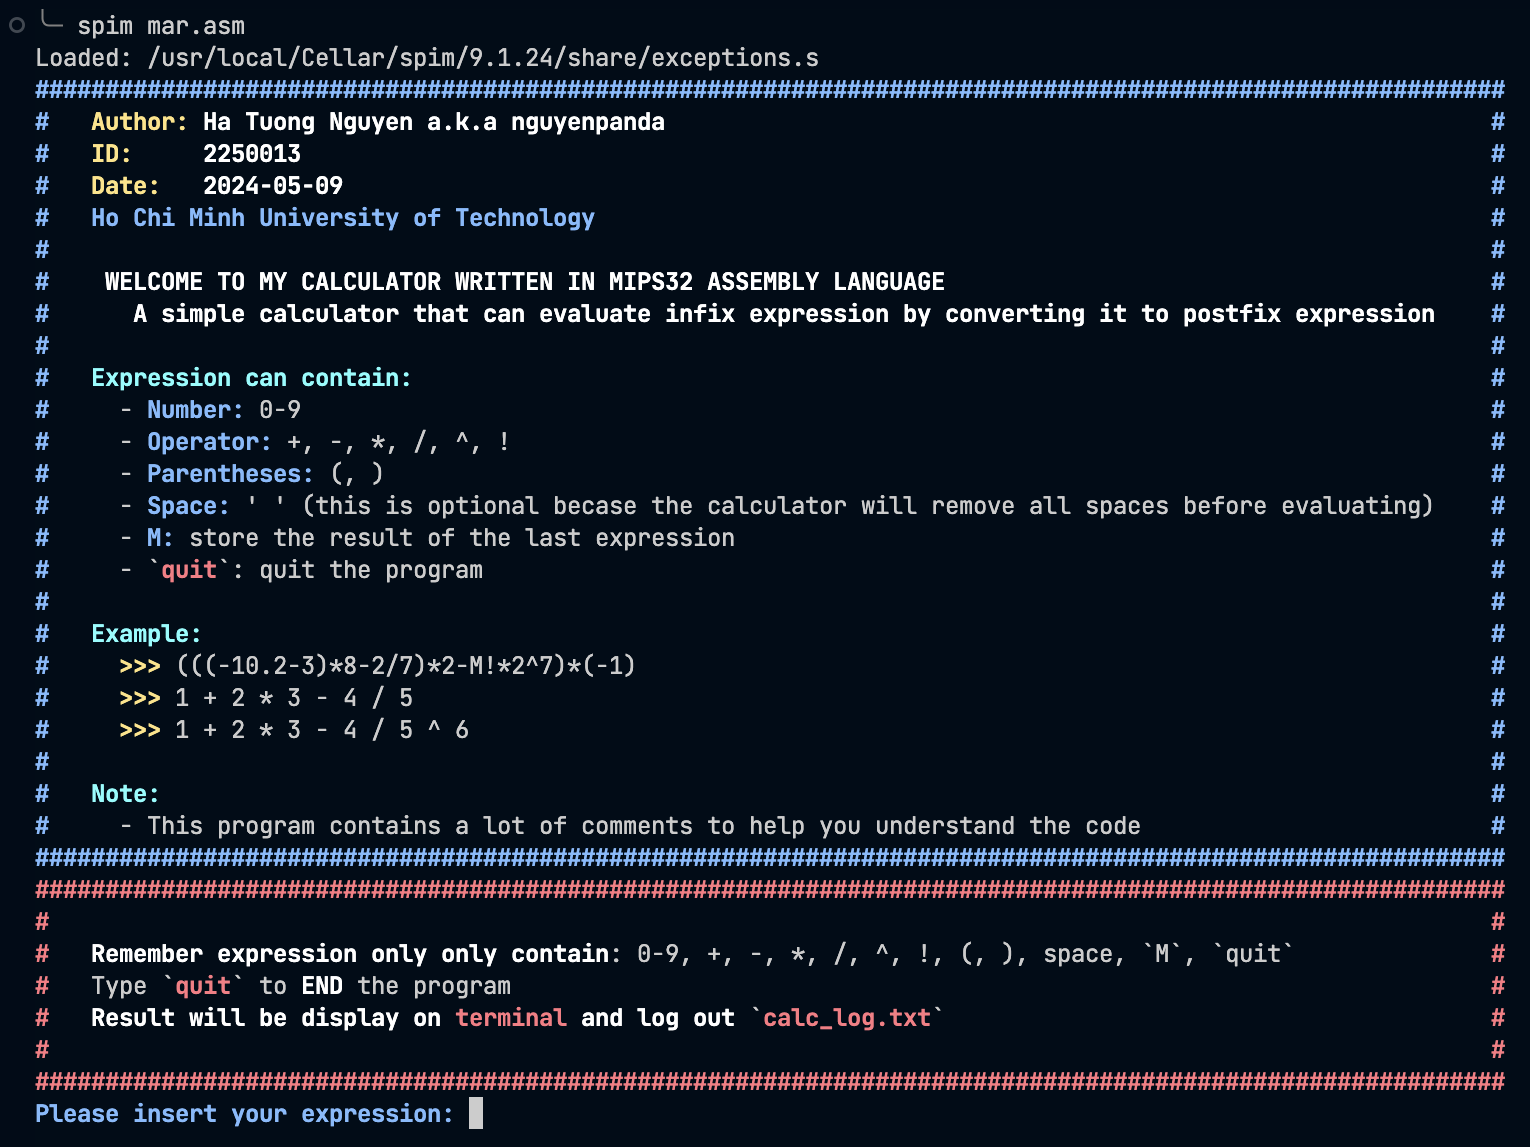
\includegraphics[width=1\textwidth]{graphics/1.Init.png}
        \caption{Starting the program}
        \label{fig:1.InitProgram}
    \end{figure}
    
    When entering an expression and pressing enter, the software will calculate and display the result of the operation. Simultaneously, it will display a red instruction frame for the next steps for the user. Meanwhile, the value of that operation will be saved in '\texttt{M}' and written to the file '\texttt{calc\_log.txt}' with \emph{16 decimal places} after the decimal point.
    
    \begin{figure}[htbp]
        \centering
        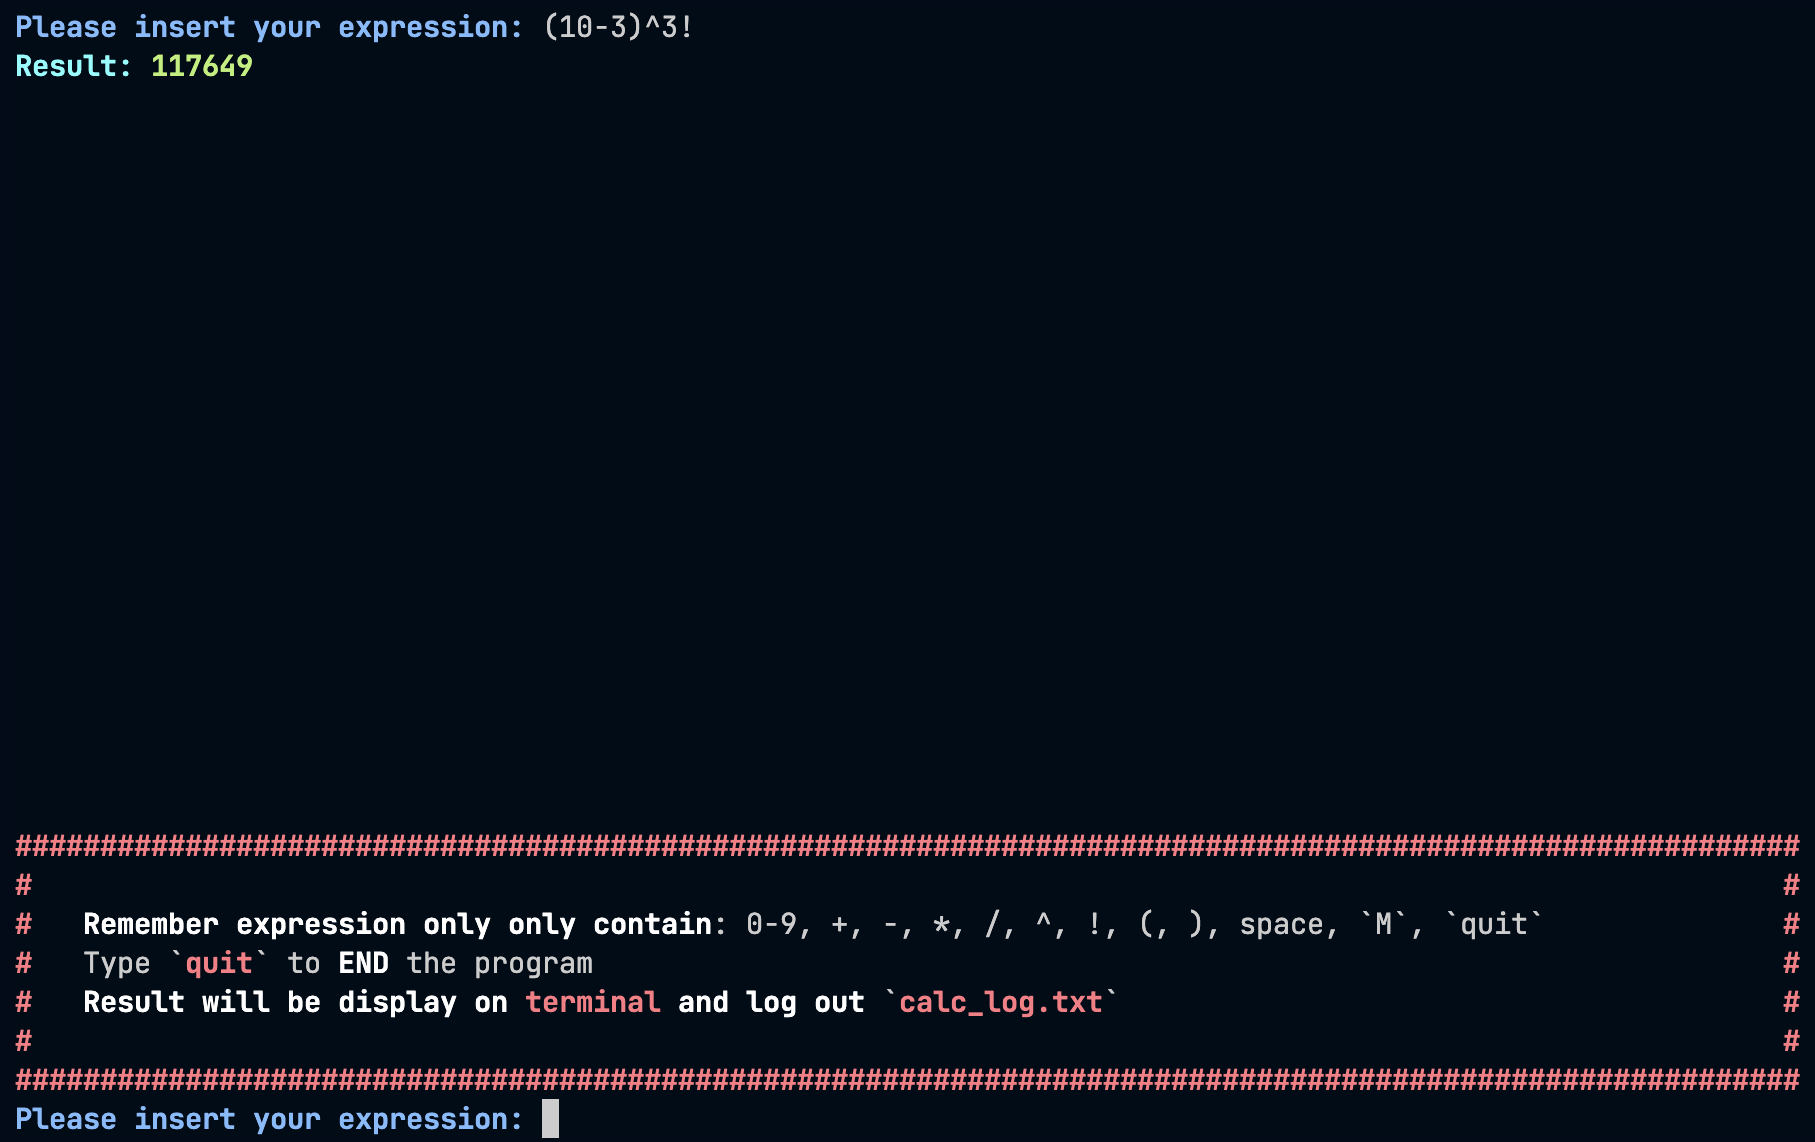
\includegraphics[width=1\textwidth]{graphics/1.AfterCalculate.png}
        \caption{After entering the first expression}
        \label{fig:1.AfterCalculate}
    \end{figure}
    
    If the user enters '\texttt{quit}', the program will terminate and notify the user that they have entered '\texttt{quit}', ending the program.
    
    \begin{figure}[htbp]
      \centering
      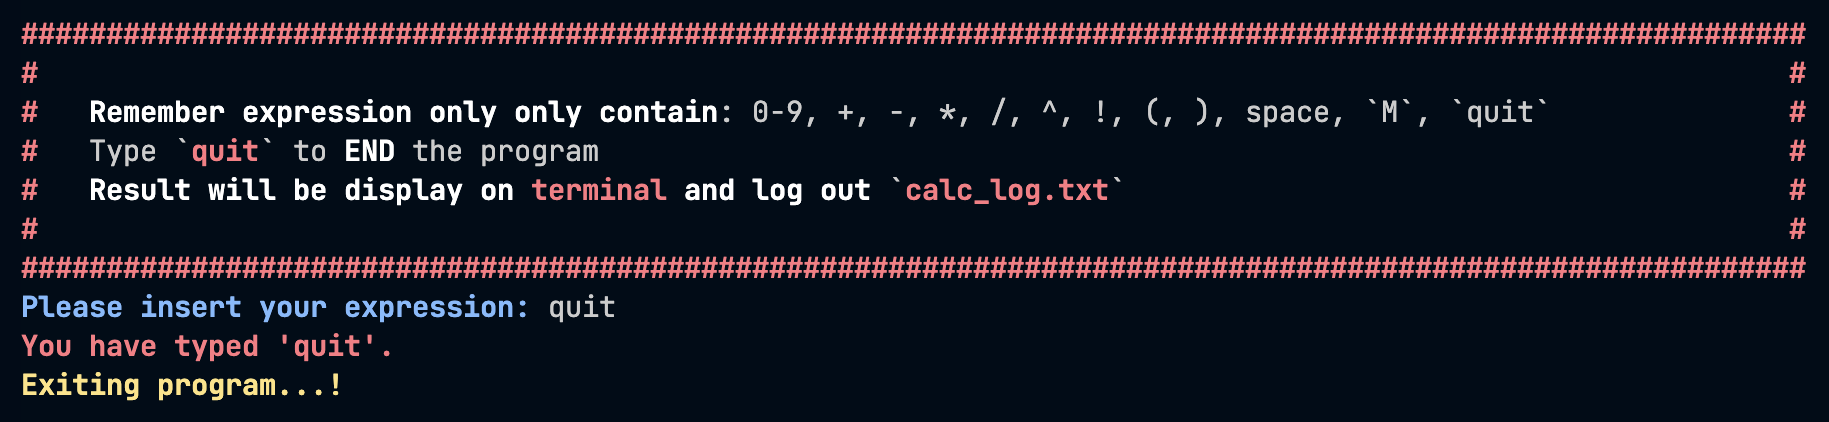
\includegraphics[width=1\textwidth]{graphics/1.Quit.png}
      \caption{User enter '\texttt{quit}'}
      \label{fig:1.EnterQuit}
    \end{figure}

\subsection{Run On Mars45}
\label{sec:1.Mars45}

    If you prefer not to run it on the terminal, you can run it on \textit{Mars45}. This is done very simply by downloading the \textit{Mars45} software from this link [\href{https://courses.missouristate.edu/kenvollmar/mars/download.htm}{Missouri State University}]. After downloading, open the file and then click \texttt{Assemble} \(\rightarrow\) \texttt{Run}.

    \begin{figure}[htbp]
        \centering
        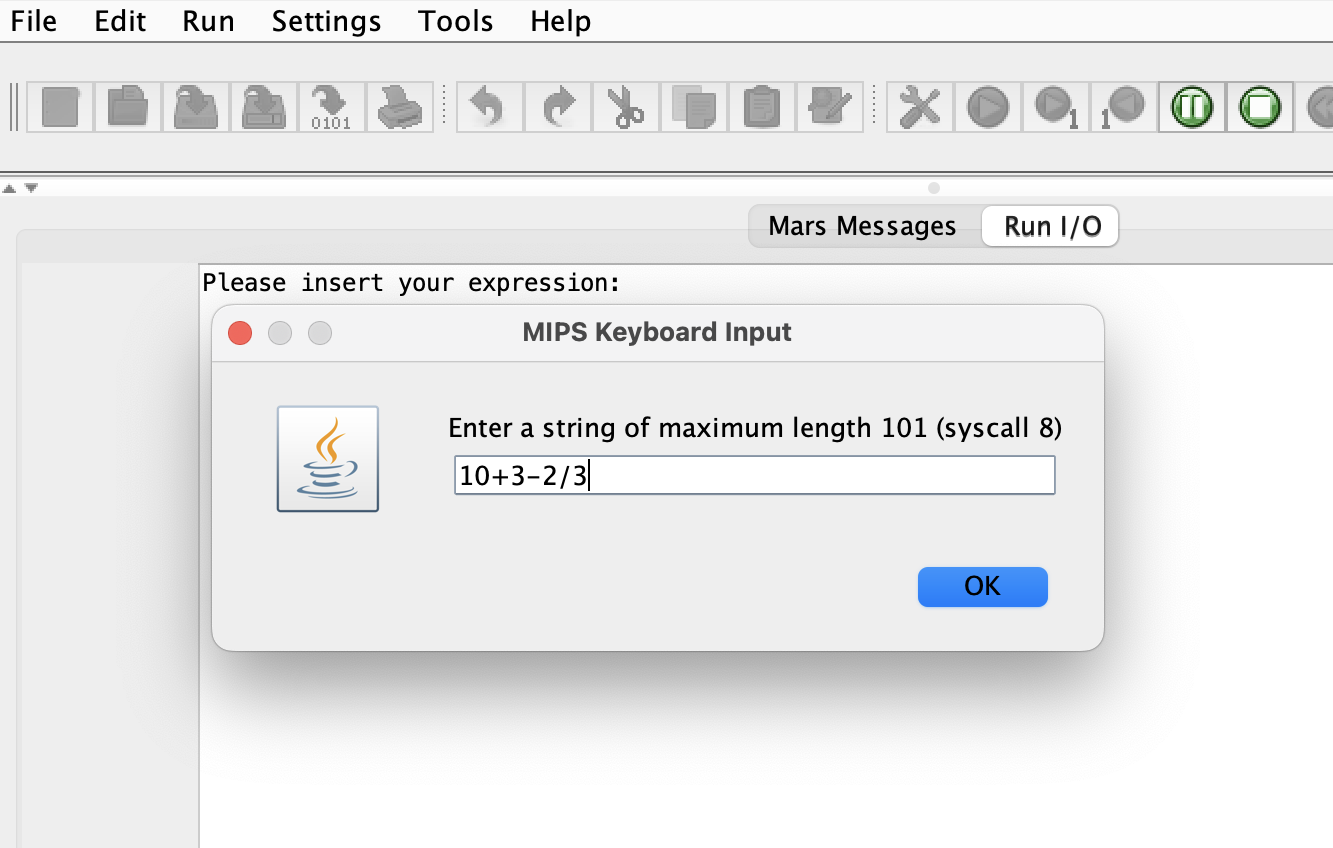
\includegraphics[width=0.6\textwidth]{graphics/1.Mars45Enter.png}
        \caption{Starting the program on \textit{Mars45}}
        \label{fig:1.MarsEnter}
    \end{figure}

    However, using \textit{Mars45} will not display the vibrant colored instruction frame because \textit{Mars45} does not support ANSII color-coded character output. This can be easily overcome by going to Settings and enabling '\texttt{Popup dialog for input syscalls}'. When running, you will see a dialog box and the result on '\texttt{Run I/O}'.

    \begin{figure}[htbp]
        \centering
        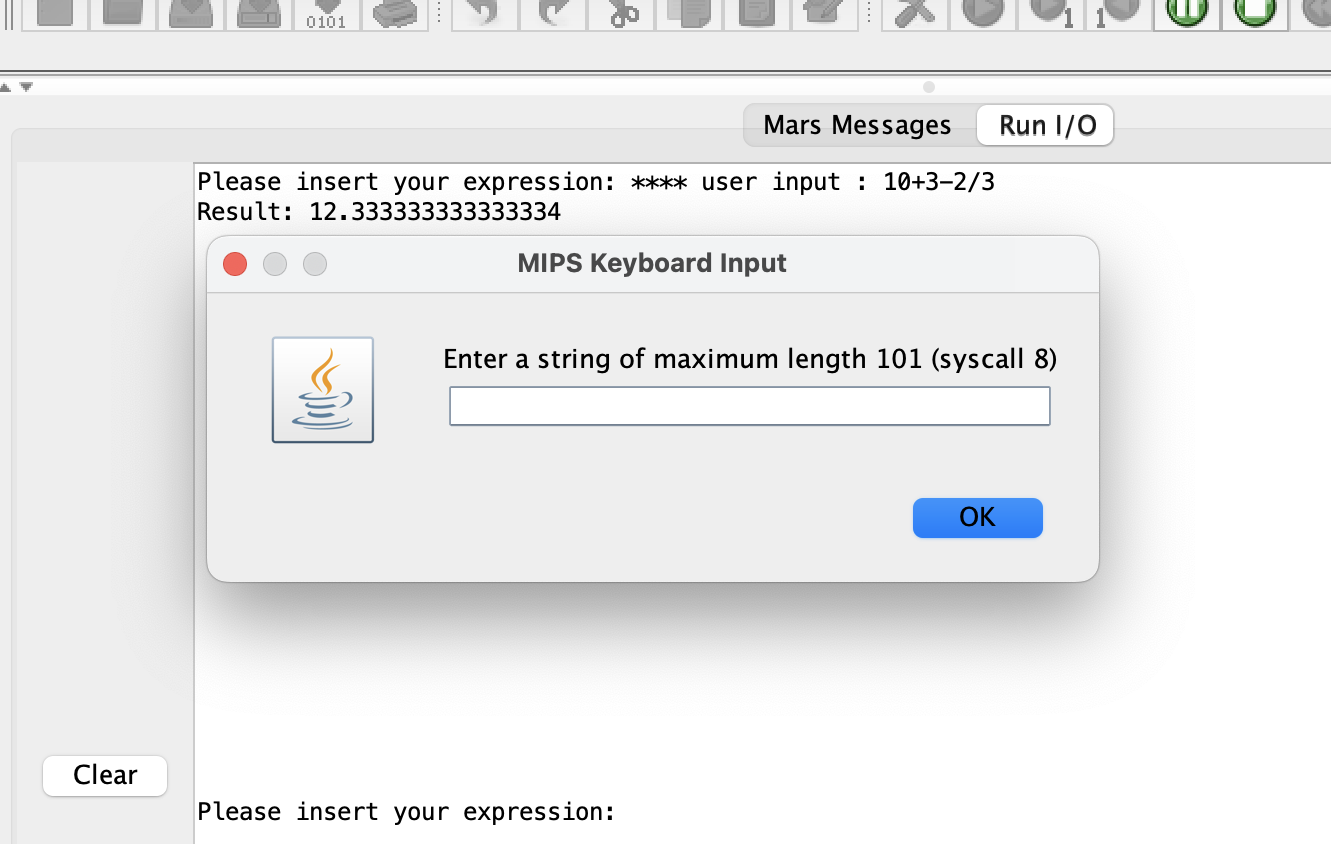
\includegraphics[width=0.6\textwidth]{graphics/1.Mars45Output.png}
        \caption{After entering the expression on \textit{Mars45}}
        \label{fig:1.MarsOutput}
    \end{figure}